% Agragar texto.
En el centro de esta historia está Arthur Morgan, el principal ejecutor y mano 
derecha de la banda de Dutch van der Linde. A diferencia de los héroes tradicionales, 
Arthur es un hombre imperfecto, moldeado por una vida de crímenes, pero que posee un 
código de honor propio. A lo largo de la narrativa, el jugador acompaña su lucha 
interna: la lealtad inquebrantable a la banda que lo crio frente a la creciente 
percepción de que el tiempo de los forajidos ha llegado a su fin.

\begin{figure}[H] % Para incertar imagen, observar la documentación en https://www.overleaf.com/learn/latex/Inserting_Images_es.
    \centering % Para centrar, 
    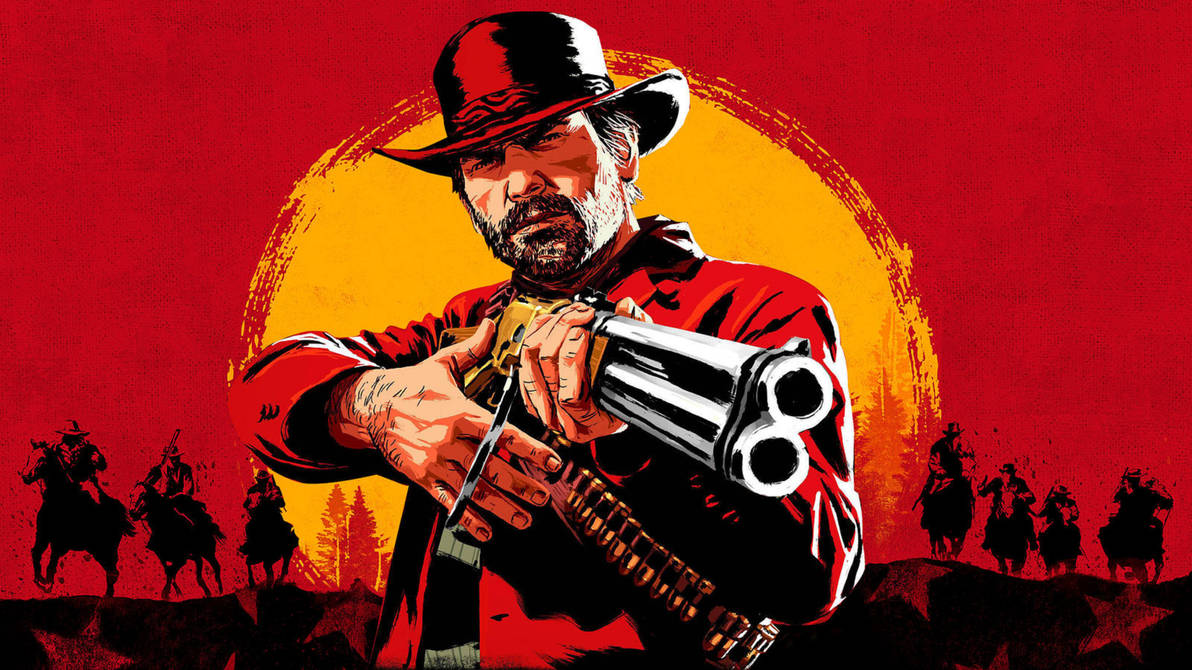
\includegraphics[width=0.6\linewidth]{Figures_Test/Arturo.jpg} % Insertar la imagen.
    \caption{Arthur Morgam} % Título imagen.
    \label{fig:img1} % Para citar la imagen posteriormente en el documneto.
\end{figure}

La dinámica de la banda funciona como una gran familia disfuncional. 
El grupo vive en campamentos, siempre huyendo y buscando un último gran golpe que 
les garantice el dinero suficiente para escapar, un sueño que se vuelve cada vez más 
inalcanzable a medida que el cerco de la ley se cierra, Figura \ref{fig:img1}. % Para referenciar figura.
